\documentclass[12pt]{article}

\usepackage{fancyhdr}
\usepackage{fullpage}
\usepackage{amsmath}
\usepackage{amsbsy}
\usepackage{amssymb}
\usepackage{amscd}
\usepackage{amsfonts}
\usepackage{amsthm}
\usepackage{supertabular}
\usepackage{graphicx}
\usepackage{verbatim}
\usepackage{epsfig}
\usepackage{xspace}
\usepackage{euscript}
\usepackage{alltt}
\usepackage{boxedminipage}
\usepackage{float}
\usepackage{times}
\usepackage{epic}
\usepackage{eepic}
\usepackage{ifthen}
\usepackage{algorithm}
\usepackage{algorithmic}
\usepackage{booktabs}
\usepackage{multirow}

\usepackage[colorlinks]{hyperref}
\usepackage[numbers,sort&compress]{natbib}
\usepackage[FIGBOTCAP,TABTOPCAP,bf,tight]{subfigure}

\usepackage[T1]{fontenc}
\usepackage{ae,aecompl}

\newcommand{\mbs}[1]{\boldsymbol{#1}}
\newcommand{\mbb}[1]{\mathbb{#1}}
\newcommand{\mbf}[1]{\mathbf{#1}}
\newcommand{\mbc}[1]{\boldsymbol{\mathcal{#1}}}

\newtheorem{proposition}{Proposition}

\def\ljump{\lbrack\!\lbrack} \def\rjump{\rbrack\!\rbrack}

\def\bA{{\mbs{A}}} \def\bB{{\mbs{B}}} \def\bC{{\mbs{C}}}
\def\bD{{\mbs{D}}} \def\bE{{\mbs{E}}} \def\bF{{\mbs{F}}}
\def\bG{{\mbs{G}}} \def\bH{{\mbs{H}}} \def\bI{{\mbs{I}}}
\def\bJ{{\mbs{J}}} \def\bK{{\mbs{K}}} \def\bL{{\mbs{L}}}
\def\bM{{\mbs{M}}} \def\bN{{\mbs{N}}} \def\bO{{\mbs{O}}}
\def\bP{{\mbs{P}}} \def\bQ{{\mbs{Q}}} \def\bR{{\mbs{R}}}
\def\bS{{\mbs{S}}} \def\bT{{\mbs{T}}} \def\bU{{\mbs{U}}}
\def\bV{{\mbs{V}}} \def\bW{{\mbs{W}}} \def\bX{{\mbs{X}}}
\def\bY{{\mbs{Y}}} \def\bZ{{\mbs{Z}}}

\def\ba{{\mbs{a}}} \def\bb{{\mbs{b}}} \def\bc{{\mbs{c}}}
\def\bd{{\mbs{d}}} \def\be{{\mbs{e}}} \def\fb{{\mbs{f}}}
\def\bg{{\mbs{g}}} \def\bh{{\mbs{h}}} \def\bi{{\mbs{i}}}
\def\bj{{\mbs{j}}} \def\bk{{\mbs{k}}} \def\bl{{\mbs{l}}}
\def\bm{{\mbs{m}}} \def\bn{{\mbs{n}}} \def\bo{{\mbs{o}}}
\def\bp{{\mbs{p}}} \def\bq{{\mbs{q}}} \def\br{{\mbs{r}}}
\def\bs{{\mbs{s}}} \def\bt{{\mbs{t}}} \def\bu{{\mbs{u}}}
\def\bv{{\mbs{v}}} \def\bw{{\mbs{w}}} \def\bx{{\mbs{x}}}
\def\by{{\mbs{y}}} \def\bz{{\mbs{z}}}

\def\balpha{{\mbs{\alpha}}}
\def\bbeta{{\mbs{\beta}}}
\def\bgamma{{\mbs{\gamma}}}
\def\bdelta{{\mbs{\delta}}}
\def\bepsilon{{\mbs{\epsilon}}}
\def\bvarepsilon{{\mbs{\varepsilon}}}
\def\bzeta{{\mbs{\zeta}}}
\def\beeta{{\mbs{\eta}}}
\def\btheta{{\mbs{\theta}}}
\def\bvartheta{{\mbs{\vartheta}}}
\def\bgamma{{\mbs{\gamma}}}
\def\bkappa{{\mbs{\kappa}}}
\def\blambda{{\mbs{\lambda}}}
\def\bmu{{\mbs{\mu}}}
\def\bnu{{\mbs{\nu}}}
\def\bxi{{\mbs{\xi}}}
\def\bomicron{{\mbs{o}}}
\def\bpi{{\mbs{\pi}}}
\def\bvarpi{{\mbs{\varpi}}}
\def\brho{{\mbs{\rho}}}
\def\bvarrho{{\mbs{\varrho}}}
\def\bsigma{{\mbs{\sigma}}}
\def\bvarsigma{{\mbs{\varsigma}}}
\def\btau{{\mbs{\tau}}}
\def\bupsilon{{\mbs{\upsilon}}}
\def\bphi{{\mbs{\phi}}}
\def\bvarphi{{\mbs{\varphi}}}
\def\bchi{{\mbs{\chi}}}
\def\bpsi{{\mbs{\psi}}}
\def\bomega{{\mbs{\omega}}}

\def\bGamma{{\mbs{\Gamma}}}
\def\bDelta{{\mbs{\Delta}}}
\def\bTheta{{\mbs{\Theta}}}
\def\bLambda{{\mbs{\Lambda}}}
\def\bXi{{\mbs{\Xi}}}
\def\bPi{{\mbs{\Pi}}}
\def\bSigma{{\mbs{\Sigma}}}
\def\bUpsilon{{\mbs{\Upsilon}}}
\def\bPhi{{\mbs{\Phi}}}
\def\bPsi{{\mbs{\Psi}}}
\def\bOmega{{\mbs{\Omega}}}

\def\dt{{\triangle t}}

\DeclareMathOperator{\tr}{tr}

\DeclareMathOperator{\divrg}{div}
\DeclareMathOperator{\grad}{grad}
\DeclareMathOperator{\curl}{curl}

\DeclareMathOperator{\Div}{Div}
\DeclareMathOperator{\Grad}{Grad}
\DeclareMathOperator{\Curl}{Curl}

\DeclareMathOperator{\dev}{dev}
\DeclareMathOperator{\vol}{vol}
\DeclareMathOperator{\Dev}{Dev}
\DeclareMathOperator{\Vol}{Vol}

% added:
\newcommand{\tensor}[1]{\ensuremath{\boldsymbol{#1}}}
\newcommand{\jump}[1]{\lbrack\!\lbrack #1 \rbrack\!\rbrack}

\numberwithin{equation}{section}
%\numberwithin{figure}{section}
%\numberwithin{subfigure}{section}

\begin{document}

%\setlength{\headheight}{15pt}
%\headsep = 4pt
%\pagestyle{fancyplain}

%\lhead
%[\fancyplain{}{\emph{A.Mota, Q.Chen, J.Foulk, J.Ostien}}]
%{\fancyplain{}{\emph{A.Mota, Q.Chen, J.Foulk, J.Ostien}}}

%\rhead
%[\fancyplain{} {\emph{Cartesian Parametrization for Material Instability}}]
%{\fancyplain{} {\emph{Cartesian Parametrization for Material Instability}}}

% Remove this in final version
%\lfoot
%[\fancyplain{}{\bf{DRAFT}}]
%{\fancyplain{}{\bf{DRAFT}}}

%\rfoot
%[\fancyplain{}{\bf{\today}}]
%{\fancyplain{}{\bf{\today}}}

\title{A Cartesian Parametrization for the Analysis of Material
  Instability}

\author{
  \Large Alejandro~Mota$^1$,
  Qiushi~Chen$^2$\thanks{Email: qiushi@clemson.edu},
  \\
  \Large James~W.~Foulk {III}$^1$,
  Jakob~T.~Ostien$^1$, Zhengshou Lai$^2$
  \\
  \\
  $^1$Mechanics of Materials Department\\
  Sandia National Laboratories\\
  Livermore CA 94550, USA\\
  \\
  $^2$Glenn Department of Civil Engineering\\
  Clemson University\\
  Clemson, SC 29631, USA\\   
}

\date{\today}

\maketitle

\begin{abstract}
  We propose a Cartesian parametrization for vectors to test for the
  loss of the ellipticity condition in the analysis of material
  instability.

  The parametrization is used to construct a tensor that is the
  acoustic tensor multiplied by a scalar factor. It is shown that both
  tensors become singular at the same time and in the same planes in
  the presence of a material instability.

  The performance of the Cartesian parametrization is compared against
  other common and uncommon parametrizations of the acoustic
  tensor. The results of these comparisons show that the Cartesian
  parametrization is more robust and more numerically efficient than
  the other tested parametrizations in general.

\end{abstract}

\section{Introduction}
\label{sec:intro}
The analysis of material instability plays an important role in the
simulation of constitutive behavior. A reliable method for the
detection of material instability is required whether one is
interested in studying the instability itself or to devise numerical
regularization methods that prevent lack of convergence once an
instability is present.

Herein we adopt the definition of material instability as the loss of
the \emph{strong ellipticity condition}, which is equivalent to the
loss of the \emph{strong Legendre-Hadamard condition} for stored
energy densities that are twice continuously differentiable
\citep{Antman:2005}.

\subsection{Previous Work}

Extensive work has been done on the subject of material
instabilities. See \citet*{Armero.Garikipati:1996} and
\citet*{Miehe.Lambrecht.Gurses:2004} for a brief historical overview
of the development of classical localization analysis, starting with
the seminal work of \citet{Hadamard:1903}, followed by
\citet{Thomas:1961}, \citet{Hill:1962}, \citet{Rice:1976} and others.

In all these works, the criterion for determining the existence of a
material instability is the loss of the strong ellipticity condition.

Assumptions \citep{Becker:2002}.

\section{General Framework}

The determination of the loss of the strong ellipticity condition for
a very general class of materials can be achieved by recourse to
incremental variational constitutive updates. Within this framework,
an incremental stress potential embodies the constitutive behavior of
the material during a time increment, including elasticity,
viscoelasticity, viscoplasticity, and rate dependence
\citep{Ortiz.Stainier:1999, Lambrecht.Miehe.Dettmar:2003,
  Miehe.Lambrecht.Gurses:2004, Weinberg.etal:2006,
  Fancello.Ponthot.Stainier:2006, Mosler.Bruhns:2010,
  Bleier.Mosler:2012}.

\subsection{Variational Constitutive Updates}

The mechanical response of the solids considered here is characterized
by a dissipation potential of the form
\begin{equation} \label{eq:power-density}
  D(\bF, \dot{\bF}, \bZ, \dot{\bZ})
  =
  \dot{A}(\bF, \bZ)
  +
  \phi(\bF, \dot{\bF}, \bZ)
  +
  \psi^*(\bZ, \dot{\bZ}),
\end{equation}
in which $A(\bF, \bZ)$ is the Helmholtz free-energy density,
$\phi(\bF, \dot{\bF}, \bZ)$ is a viscous potential, $\psi^*(\bZ,
\dot{\bZ})$ is a dual kinetic potential or dissipation function, $\bF$
is the deformation gradient and $\bZ$ is a collection of suitable
internal variables that describe the state of the material at a given
point. The first Piola-Kirchhoff stress and the conjugate
thermodynamic forces to $\bZ$ are given by
\begin{equation} \label{eq:1PKstress-and-Y}
  \bP
  =
  \frac{\partial D}{\partial \dot{\bF}}(\bF, \dot{\bF}, \bZ, \dot{\bZ})
  =
  \frac{\partial A}{\partial \bF}(\bF, \bZ)
  +
  \frac{\partial \phi}{\partial \dot{\bF}}(\bF, \dot{\bF}, \bZ),
  \quad
  \bY = - \frac{\partial A}{\partial \bZ} (\bF, \bZ),
\end{equation} 
respectively. In order to ensure a variational structure, we have
postulated the existence of a dual kinetic potential or dissipation
function $\psi^*(\bZ, \dot{\bZ})$ such that
\begin{equation} \label{eq:dual-kinetic-potential}
  \bY = \frac{\partial \psi^*}{\partial \dot{\bZ}} (\bZ, \dot{\bZ}).
\end{equation}
Next, we minimize the dissipation potential \eqref{eq:power-density}
with respect to the internal variable rates as
\begin{equation}
  \begin{split}
    \inf_{\dot{\bZ}} [ D(\bF, \dot{\bF}, \bZ, \dot{\bZ}) ]
    =
    &
    \inf_{\dot{\bZ}}
    \left[
      \dot{A}(\bF, \bZ)
      +
      \psi^*(\bZ, \dot{\bZ})
    \right] +
    \phi(\bF, \dot{\bF}, \bZ),
    \\
    =
    &
    \inf_{\dot{\bZ}}
    \left[
      \frac{\partial A}{\partial \bF}(\bF, \bZ) : \dot{\bF}
      +
      \frac{\partial A}{\partial \bZ}(\bF, \bZ) \cdot \dot{\bZ}
      +
      \psi^*(\bZ, \dot{\bZ})
    \right] +
    \phi(\bF, \dot{\bF}, \bZ),
  \end{split}
\end{equation}
which in turn leads to Biot's equation for standard dissipative systems
\begin{equation} \label{eq:Biots-equation}
  \frac{\partial A}{\partial \bZ} (\bF, \bZ)
  +
  \frac{\partial \psi^*}{\partial \dot{\bZ}} (\bZ, \dot{\bZ})
  =
  \mathbf{0}.
\end{equation}
Approximate solutions to this equation may be found by recourse to the
incremental energy density function for a time increment $t \in [t_n,
t_{n+1}]$
\begin{equation} \label{incremental-energy-density}
  w(\bF_{n+1}, \bZ_{n+1}) := 
  \int_{t_n}^{t_{n+1}}
  \left[
    \dot{A}(\bF, \bZ)
    +
    \phi(\bF, \dot{\bF}, \bZ)
    +
    \psi^*(\bZ, \dot{\bZ})
  \right]
  \, dt,
\end{equation}
in which the integral is evaluated using a midpoint-like rule
as follows
\begin{equation} \label{incremental-energy-density-mid-point}
  \begin{split}
    w(\bF_{n+1}, \bZ_{n+1}) \approx
    &
    A(\bF_{n+1}, \bZ_{n+1}) - A(\bF_n, \bZ_n) +
    \\
    &
    \triangle t
    \left[
      \phi
      \left(
        \bF_{n+\alpha}, \frac{\triangle \bF}{\triangle t}, \bZ_{n+\alpha}
      \right)
      +
      \psi^*
      \left(
        \bZ_{n+\alpha}, \frac{\triangle \bZ}{\triangle t}
      \right)
    \right].
  \end{split}
\end{equation}
with
\begin{equation} \label{eq:increments}
  \triangle t := t_{n+1} - t_n,
  \quad
  \triangle \bF := \bF_{n+1} \bF_n^{-1},
  \quad
  \triangle \bZ := \bZ_{n+1} - \bZ_n,
\end{equation}
and
\begin{equation} \label{eq:mid-values}
  \begin{split}
    \bF_{n+\alpha} & := \exp[(1 - \alpha) \log \bF_n + \alpha \log \bF_{n+1}],
    \\
    \bZ_{n+\alpha} & := (1 - \alpha) \bZ_n + \alpha \bZ_{n+1},
  \end{split}
\end{equation}
where $\alpha$ is an algorithmic parameter. In order to obtain an
explicit scheme, we choose $\alpha = 0$. Next, we define the
incremental stress potential as
\begin{equation} \label{eq:incremental-stress-potential}
  \begin{split}
    W(\bF_{n+1})
    :=
    &
    \inf_{\bZ_{n+1}}[w(\bF_{n+1}, \bZ_{n+1})]
    \\
    =
    &
    \inf_{\bZ_{n+1}}
    \left[
      A(\bF_{n+1}, \bZ_{n+1}) - A(\bF_n, \bZ_n)
      +
      \triangle t
      \psi^*\left(\bZ_n, \frac{\triangle \bZ}{\triangle t}\right)
    \right]
    +
    \\
    &
    \triangle t
    \phi\left(\bF_n, \frac{\triangle \bF}{\triangle t}, \bZ_n\right).
  \end{split}
\end{equation}
This minimization provides an optimal path for the internal variables
$\bZ$ in the time increment $t \in [t_n, t_{n+1}]$. Furthermore, the
Euler-Lagrange equation corresponding to
\eqref{eq:incremental-stress-potential} is
\begin{equation} \label{eq:Biots-equation-discrete}
  \frac{\partial A}{\partial \bZ_{n+1}}(\bF_{n+1}, \bZ_{n+1})
  +
  \triangle t
  \frac{\partial \psi^*}{\partial \bZ_{n+1}}
  \left(\bZ_n, \frac{\triangle \bZ}{\triangle t}\right)
  =
  \mathbf{0}.
\end{equation}
which is a discrete version of Biot's equation
\eqref{eq:Biots-equation} \citep{Miehe:Schotte:Lambrecht:2002}. The
incremental first Piola-Kirchhoff stress and tangent moduli can be
computed in turn as
\begin{equation} \label{eq:incremental-stress-moduli}
  \bP_{n+1} := \frac{\partial W}{\partial \bF} (\bF_{n+1}),
  \quad
  \mbb{C}_{n+1} := \frac{\partial^2 W}{\partial \bF^2} (\bF_{n+1}),
\end{equation}
respectively. Thus, by using variational constitutive updates, the
stress and the tangent moduli can be derived from the
hyperleastic-like potential \eqref{eq:incremental-stress-potential}
for a very general class of constitutive behavior that may include
viscosity and rate dependence. This in turn provides the means to
apply the classical analysis tools that are used in hyperelasticity
for complex materials as well.

\subsection{The Strong Ellipticity Condition}

For simplicity in notation and unless otherwise stated, henceforth we
omit the time indices $n$ and $n+1$ with the understating that further
developments take place at time $t_{n+1}$.

The ellipticity condition can be expressed as
\begin{equation} \label{eq:strong-ellipticity}
  (\bm \otimes \bn) : \mbb{C} : (\bm \otimes \bn) \ge 0,
  \quad
  \forall \, \bm, \bn \in \mbb{R}^3.
\end{equation}
If the condition holds strictly for non-zero vectors $\bm$ and $\bn$,
then it is called the strong ellipticity condition
\citep{Hadamard:1903, Truesdell.Noll:2004,
  Miehe.Lambrecht.Gurses:2004}. It is customary to \emph{assume} that
$\bm$ and $\bn$ are unit vectors, \emph{i.e.} $\bm, \bn \in S^2$ where
$S^2 := \{ \bt \in \mbb{R}^3 \, | \, \| \bt \| = 1\}$ is the unit
sphere. Define the acoustic tensor as
\begin{equation} \label{eq:acoustic-tensor}
  \bA := \bn \cdot \mbb{C} \cdot \bn
  \quad \text{or} \quad
  A_{jk} := n_i C_{ijkl} n_l,
  \quad
  \bn \in S^2,
\end{equation}
then the strong ellipticity condition becomes
\begin{equation} \label{eq:acoustic-ellipticity}
  \bm \cdot \bA \cdot \bm > 0, \quad \bm \in S^2.
\end{equation}
In order to satisfy the strong ellipticity condition, the acoustic
tensor must be positive definite. Therefore,
\eqref{eq:strong-ellipticity} and \eqref{eq:acoustic-ellipticity}
reduce to
\begin{equation} \label{eq:acoustic-determinant}
  \det \bA > 0,
\end{equation}
which provides a method to determine the onset of a material
instability.

\subsection{Bifurcation}

By using the strong ellipticity condition
\eqref{eq:strong-ellipticity} or its equivalent with the acoustic
tensor \eqref{eq:acoustic-determinant}, the detection of bifurcation
or loss of ellipticity in the material is fully characterized by its
fourth-order tangent moduli \eqref{eq:incremental-stress-moduli}. The
onset of bifurcation is then posed as a minimization problem.  First
we assume that the normal vector $\bn$ is parametrized by a set of
parameters $\bq$, thus turning the determinant of the acoustic tensor
$\det \bA$ into a function of $\bq$.  Then the determinant of the
acoustic tensor $\det \bA(\bq)$ is minimized with respect to
$\bq$. Thus the loss of strong ellipticity may be stated as
\begin{equation} \label{eq:minimization-determinant}
  f(\bq) := \det \bA(\bq),
  \quad
  \min_{\bq} f(\bq) = 0,
  \quad
  \bn(\bq) \in S^2.
\end{equation}
If the determinant function $f(\bq)$ is differentiable, the
minimization problem can be rewritten equivalently as
\begin{equation}\label{eq:minimization-derivative}
  \frac{\partial f}{\partial \bq}(\bq) = \mathbf{0},
\end{equation}
which can be solved by standard numerical optimization techniques,
\emph{e.g.} a Newton-type iterative procedure.

\section{Parametrizations for Bifurcation Analysis}
\label{sec:parametrizations}

Efficient computation of the minimization problem
\eqref{eq:minimization-derivative} requires a careful choice of the
parametrization for the normal vector $\bn(\bq) \in S^2$, which is
equivalent to select a parametrization for the unit sphere. This
choice has a significant effect on the complexity of the determinant
function $f(\bq)$ and its derivatives with respect to $\bq$ needed to
solve the optimization problem. Herein, five different options are
explored. The first four (spherical, stereographic, projective,
tangent) are indeed parametrizations of the unit sphere.  The last
parametrization, which we term Cartesian, relaxes the restriction that
the normal vector be an element of the unit sphere. We describe the
parametrizations in detail next, assuming that a Cartesian frame of
reference originates from the center of each one.

\subsection{Spherical Parametrization}
\label{subsec:spherical}

Elements $\bn$ of the unit sphere $S^2$ are simply parametrized by
their spherical coordinates with polar angle $\varphi \in [0, \pi]$,
azimuthal angle $\theta \in [0, \pi]$ and radial distance $r = \| \bn
\| = 1$. The reduced range in the angle $\theta$ is due to symmetry of
the bifurcation condition, as for this purpose $\bn = - \bn$, see
Figure~\ref{fig:spherical}. In terms
of the canonical basis
\begin{equation}
  \bn(\varphi, \theta)
  :=
  \begin{Bmatrix}
    \sin\varphi \sin\theta
    \\
    \cos\varphi
    \\
    \sin\phi \cos\theta
  \end{Bmatrix}.
\end{equation}

\subsection{Stereographic Parametrization}
\label{subsec:stereographic}

The unit sphere is parametrized with the aid of an equatorial plane as
shown in Figure~\ref{fig:stereographic}.  Consider a point $P$ that is
both on this plane and on a line that passes through the north pole
$Q$ of the sphere and the tip of the vector $\bn$. The Cartesian
coordinates $x$ and $y$ of $P$ provide the desired parametrization,
which can be easily derived by finding the intersection of the line
and the sphere. The upper hemisphere can be ignored due to the
symmetry of the bifurcation condition, thus avoiding the singularity
in parametrizing a normal vector that points to the north pole
$Q$. The normal vector $\bn$ in terms of the canonical basis is
\begin{equation}
  \bn(x,y)
  := 
  \begin{Bmatrix}
    \frac{\displaystyle 2x}{\displaystyle x^2+y^2+1}
    \\[0.9em]
    \frac{\displaystyle 2y}{\displaystyle x^2+y^2+1}
    \\[0.9em]
    \frac{\displaystyle x^2+y^2-1}{\displaystyle x^2+y^2+1}
  \end{Bmatrix}.
\end{equation}

\subsection{Projective Parametrization}
\label{subsec:projective}

In the projective parametrization, the norm of the position vector of
a point $P$ with respect to the center of the sphere is constrained to
obtain a unit vector $\bn$ \citep{Ortiz.Leroy.Needleman:1986}. This is
equivalent to project the point $P$ onto the unit sphere $S^2$, as
shown in Figure~\ref{fig:projective}.  The normalization is effected
by means of a constraint enforced by a Lagrange multiplier as
\begin{equation}
  \bn(x,y,z)
  := 
  \begin{Bmatrix}
    x
    \\
    y
    \\
    z
  \end{Bmatrix},
  \quad
  \text{subjected to}~x^2+y^2+z^2 = 1.
\end{equation}

\subsection{Tangent Parametrization}
\label{subsec:tangent}

This parametrization of the unit sphere is defined by a tangent plane
\citep{Simo.Fox:1989}. Let $\bu\in \mbb{R}^3$ be the position vector
of the point $P$ in the tangent plane with respect to the contact
point $Q$ between the sphere and the plane, then let $\be \in S^2$ be
the position vector of the contact point $Q$ with respect to the
center of the sphere $O$, as shown in Figure~\ref{fig:tangent}. Define
a rotation vector $\btheta := \be \times \bu$, then the rotation angle
is $\theta := \| \btheta \| \equiv \| \bu \|$. Let also
$\check{\btheta} \in so(3)$ be the skew-symmetric tensor such that
$\check{\btheta} \cdot \bv \equiv \btheta \times \bv \ \forall \ \bv
\in \mbb{R}^3$. The expression for the exponential map for
$\check{\btheta}$ is
\begin{equation}
  \exp \check{\btheta}
  :=
  \begin{cases}
    \bI \in SO(3),
    &
    \text{ if }\theta = 0;
    \\
    \displaystyle{
      \bI + \frac{\sin \theta}{\theta} \check{\btheta} +
      \frac{(1 - \cos \theta)}{\theta^2} \check{\btheta}^2 \in SO(3),
    }
    &
    \text{ if }\theta > 0;
  \end{cases}
  \label{eq:Rodrigues-formula}
\end{equation}
which is often accredited to Rodrigues
\citep{Gallier:2011}. Next define
\begin{equation}
  \exp_{\be} \bu
  :=
  \exp \check{\btheta} \cdot \be
  =
  \cos \theta \be + \frac{\sin \theta}{\theta}
  \bu \in S^2.
\end{equation}
The parametrization follows immediately by setting the contact point
$Q$ to the north pole of the sphere, \emph{i.e.} $\be = [0,0,1]^T$ and
$\bu = [x,y,0]^T$ with the normal vector $\bn$ given by
\begin{equation}
  \bn
  =
  \exp_{\be} \bu \in S^2.
\end{equation}
which leads to a more explicit representation for the normal vector in
the canonical basis as
\begin{equation}
  \bn(x,y)
  := 
  \begin{Bmatrix}
    \frac{\displaystyle x \sin \sqrt{x^2+y^2}}{\displaystyle \sqrt{x^2+y^2}}
    \\[0.9em]
    \frac{\displaystyle y \sin \sqrt{x^2+y^2}}{\displaystyle \sqrt{x^2+y^2}}
    \\[0.9em]
    \cos \sqrt{x^2+y^2}
  \end{Bmatrix}.
\end{equation}

\subsection{Cartesian Parametrization}
\label{subsec:Cartesian}

The strong ellipticity condition
\begin{equation}
  (\bu \otimes \bv) : \mbb{C} : (\bu \otimes \bv) > 0,
  \quad
  \forall \, \bu, \bv \in \mbb{R}^3 \setminus \{\mathbf{0}\}
\end{equation}
only requires that the vectors $\bu$ and $\bv$ be non-zero. Thus, the
condition that they belong to the unit sphere $S^2$ may be relaxed. In
analogy to the classical acoustic tensor \eqref{eq:acoustic-tensor},
define
\begin{equation} \label{eq:Cartesian-acoustic-tensor}
  \bB := \bv \cdot \mbb{C} \cdot \bv
  \quad \text{or} \quad
  B_{jk} := v_i C_{ijkl} v_l,
  \quad
  \bv \in \mbb{R}^3 \setminus \{\mathbf{0}\},
\end{equation}
thus the strong ellipticity condition may be expressed as
\begin{equation} \label{eq:Cartesian-acoustic-ellipticity}
  \bu \cdot \bB \cdot \bu > 0,
  \quad
  \bu \in \mbb{R}^3 \setminus \{\mathbf{0}\}.
\end{equation}
As in \eqref{eq:acoustic-determinant}, the strong ellipticity
condition becomes
\begin{equation} \label{Cartesian-acoustic-determinant}
  \det \bB > 0.
\end{equation}

\begin{proposition}
  The tensor $\bB$ from \eqref{eq:Cartesian-acoustic-tensor} leads to
  the same bifurcation condition than the acoustic tensor $\bA$ from
  \eqref{eq:acoustic-tensor}.
\end{proposition}

\begin{proof}
  Introduce the bijective map $g : \mbb{R}^3 \setminus \{\mathbf{0}\}
  \mapsto S^2 \times \mbb{R}^+$ that allows the representation of
  nonzero vectors in $\mbb{R}^3$ as unit vectors in the unit sphere
  (direction) and the corresponding nonzero norm (magnitude). Then
  define
  \begin{equation}
    \bv \in \mbb{R}^3 \setminus \{\mathbf{0}\},
    \quad
    v := \| \bv \| \in \mbb{R}^+,
    \quad
    \bn := \frac{\bv}{v} \in S^2,
  \end{equation}
  therefore from \eqref{eq:acoustic-ellipticity} and
  \eqref{eq:Cartesian-acoustic-ellipticity}
  \begin{equation} \label{eq:Cartesian-from-acoustic}
      \bB(v, \bn)
      =
      v^2 \bA(\bn)
      \quad \text{and} \quad
      \det \bB(v, \bn) = v^6 \det \bA(\bn).
  \end{equation}
  Now let the bifurcation condition for $\bA$ be
  \begin{equation}
    \min_{\bn} \det \bA(\bn) = 0,
    \quad
    \ba := \arg \min_{\bn} \det \bA(\bn) \in S^2,
    \quad
    \det \bA(\bn) > 0 \, \forall \, \bn \neq \ba,
  \end{equation}
  then it follows from \eqref{eq:Cartesian-from-acoustic} that
  \begin{equation}
    \det \bB(s, \ba) = 0,
    \quad
    \det \bB(s, \bn) > 0,
    \quad \forall \, \bn \neq \ba
    \text{ and } \forall \, s \in \mbb{R}^+,
  \end{equation}
  which means that
  \begin{equation}
    \min_{v, \bn} \det \bB(v, \bn) = 0,
    \quad
    \{s, \ba\} := \arg \min_{v, \bn} \det \bB(v, \bn)
    \,
    \forall \, s \in \mbb{R}^+,
  \end{equation}
  as required.
\end{proof}

In order to remove the multiple minima associated with the arbitrary
value of the scalar parameter $s$ and obtain a parametrization, we
restrict the range of the Cartesian coordinates such that $x,y,z \in
[-1,1]$ and set the normal vector to
\begin{equation}
  \bv(x,y,z)
  :=
  \begin{cases}
    [x,y,1]^T,
    &
    \text{ if }x \in [-1,1] \text{ and } y \in [-1,1);
    \\
    [1,y,z]^T,
    &
    \text{ if }y \in [-1,1] \text{ and } z \in [-1,1);
    \\
    [x,1,z]^T,
    &
    \text{ if }z \in [-1,1] \text{ and } x \in [-1,1);
    \\
    [1,1,1]^T,
    &
    \text{ otherwise }.
  \end{cases}
\end{equation}
This confines the normal vector to the cube of side length $2$
centered at the origin as shown in Figure~\ref{fig:Cartesian}. Only
three faces of the cube need to be considered due to the symmetry of
the bifurcation condition.

\begin{figure}[htbp]
  \begin{center}
    \unitlength=1.0mm
    \subfigure[Spherical]{
      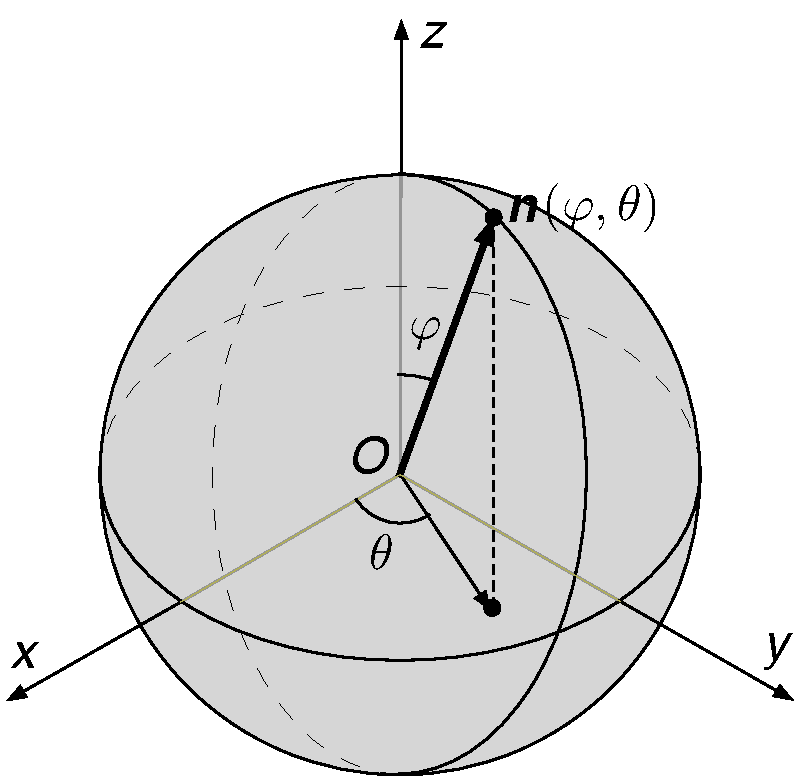
\includegraphics[width=67mm]{figs/spherical.pdf}
      \label{fig:spherical}
    }
    \subfigure[Stereographic]{
      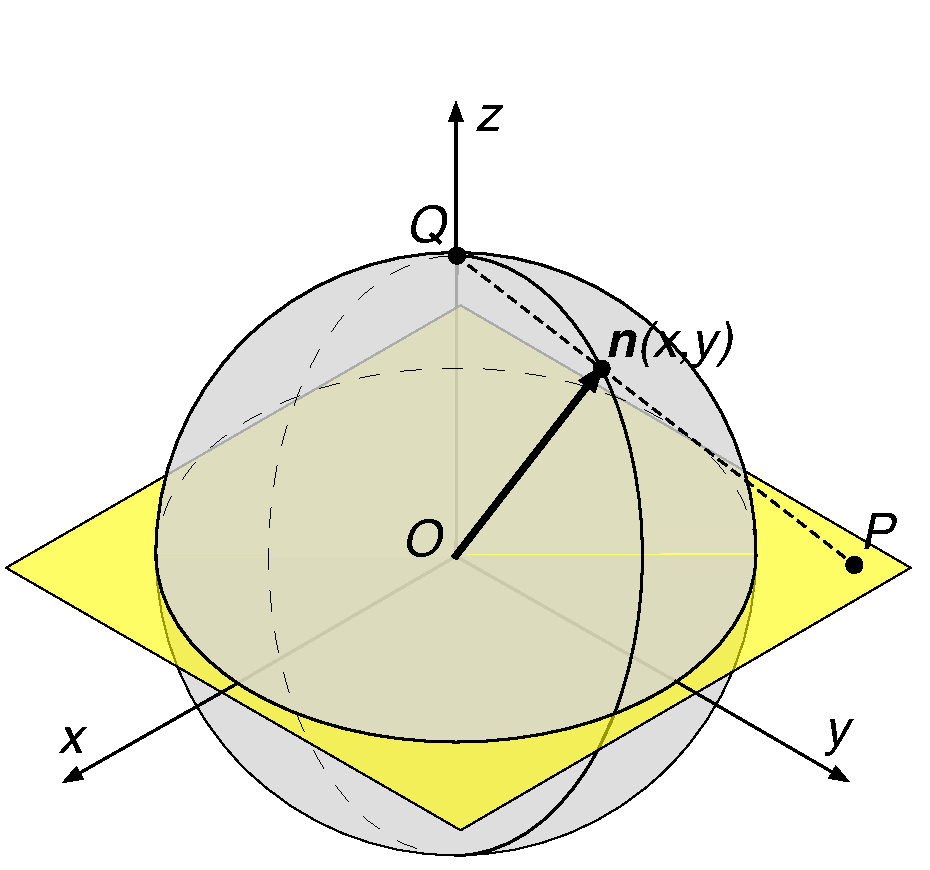
\includegraphics[width=67mm]{figs/stereographic.pdf}
      \label{fig:stereographic}
    }
    \subfigure[Projective]{
      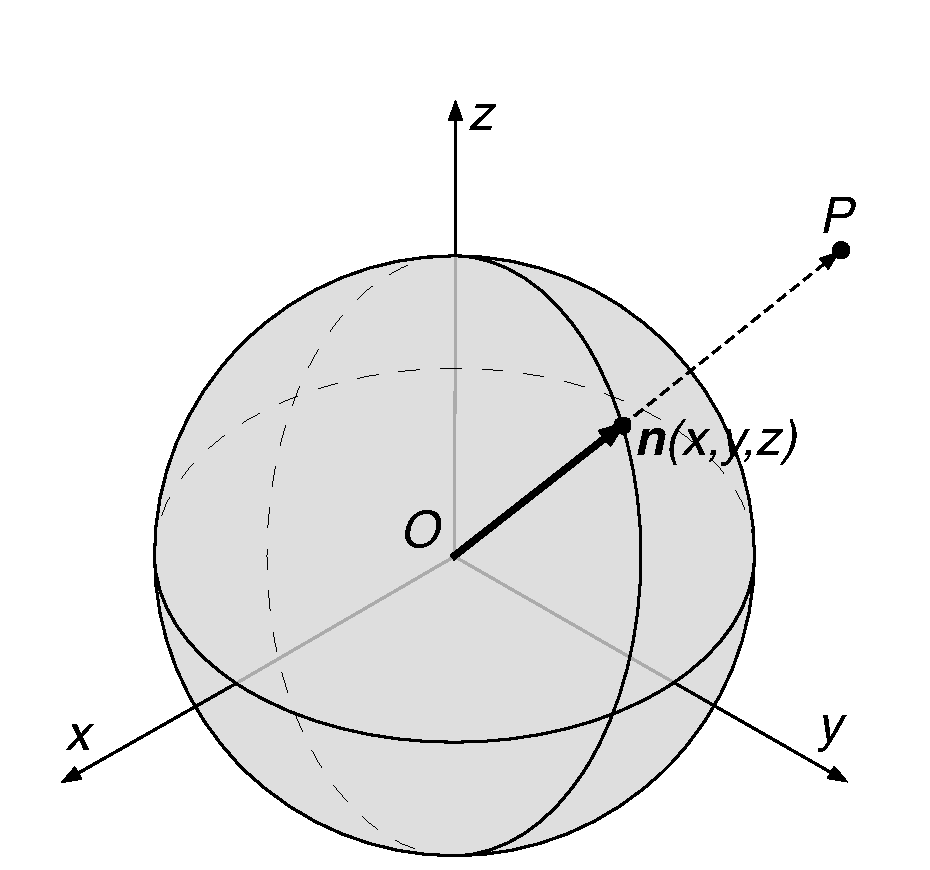
\includegraphics[width=67mm]{figs/projective.pdf}
      \label{fig:projective}
    }
    \subfigure[Tangent]{
      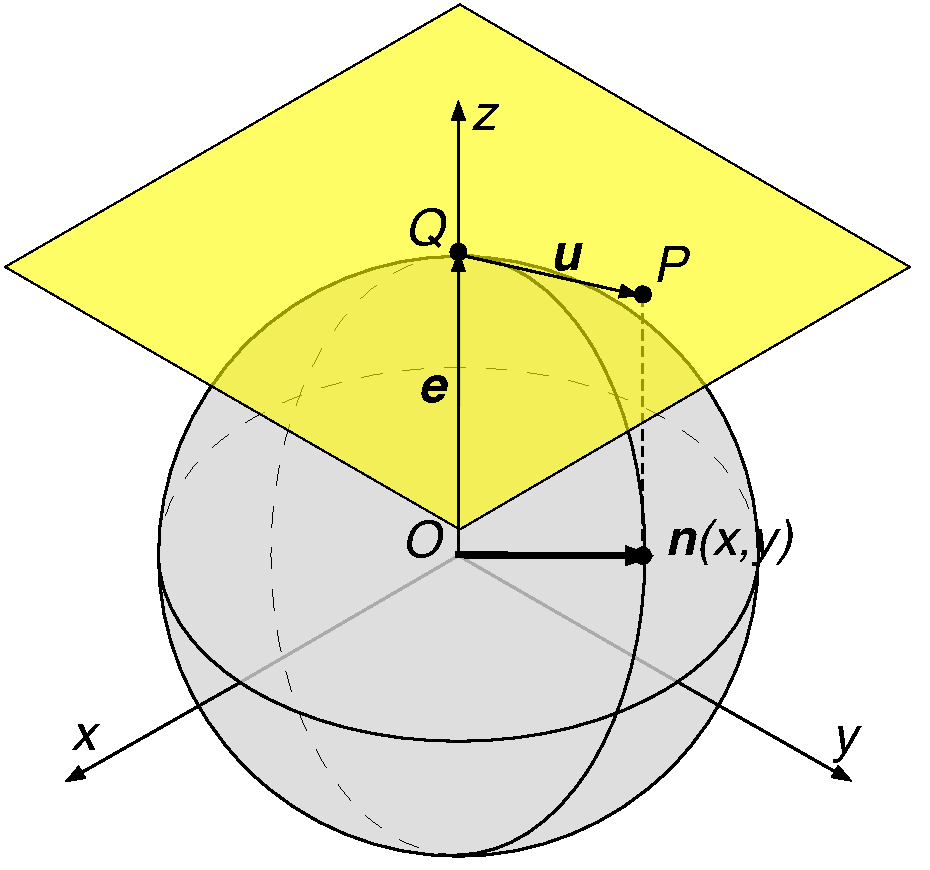
\includegraphics[width=67mm]{figs/tangent.pdf}
      \label{fig:tangent}
    }
    \subfigure[Cartesian]{
      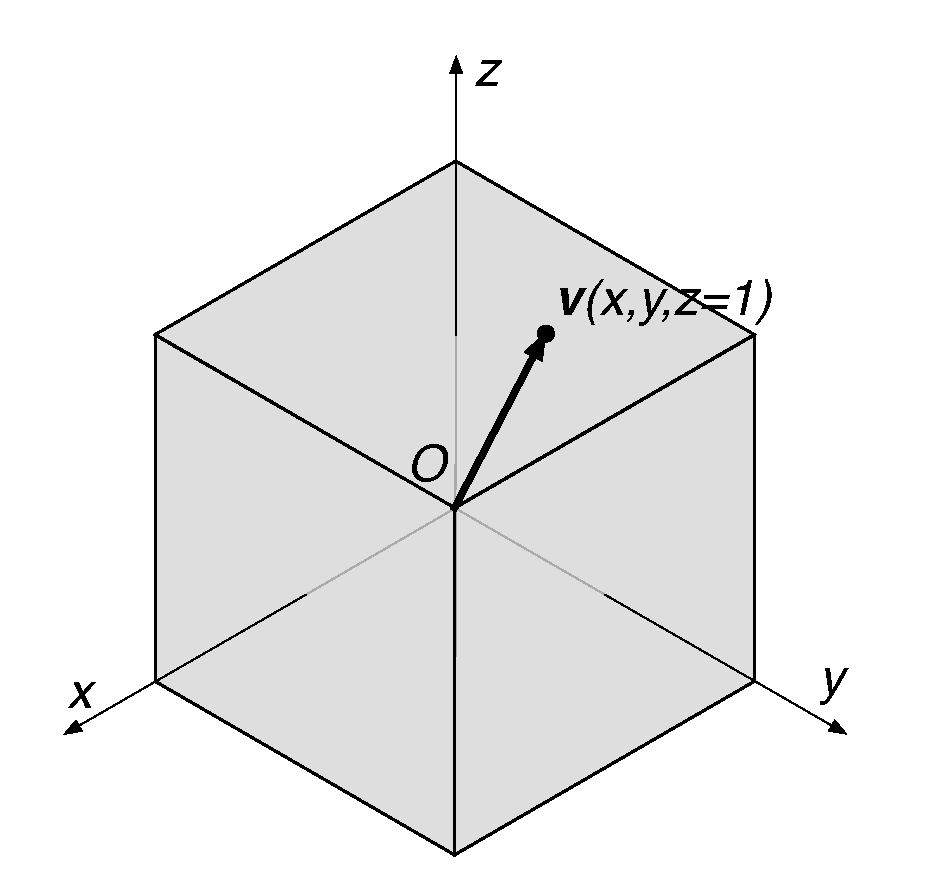
\includegraphics[width=67mm]{figs/cartesian.pdf}
      \label{fig:Cartesian}
    }
    \caption{Parametrizations.}
    \label{fig:parametrizations}
  \end{center}
\end{figure}

\section{Bifurcation Detection}

Within an incremental update setting, the detection of the bifurcation
condition for each time increment using any of the parametrizations
just described may be effected by the following procedure:

\begin{itemize}
  
\item An initial coarse sampling is performed over the parametric
  space for $\bq$ for the normal vector $\bn \in S^2$ or $\bv \in
  \mbb{R}^3 \setminus \{\mathbf{0}\}$ associated with the
  parametrization. This leads to a coarse estimate of the determinant
  function $f(\bq)$.
  
\item The coarse estimate is used to initiate a Newton-type iterative
  procedure to find a better approximation to the minimum.


\end{itemize}

This simple procedure may not yield estimates of the bifurcation
condition that are accurate enough. One way to improve the solution is
to introduce adaptive time increments. Define
\begin{equation} \label{eq:general-minimization-problem}
  \mu_n := \min_{\bq} f_n(\bq) = \min_{\bq} \det \bB_n(\bq)
\end{equation}
where the tensor $\bB_n(\bq)$ may be either the one from
\eqref{eq:acoustic-tensor} or the one from
\eqref{eq:Cartesian-acoustic-tensor}, depending of the parametrization
in use, and the index $n$ indicates that the evaluation occurs at time
$t_n$. Assume that $\mu_n > 0$, $\mu_{n+1} < 0$ and $\mu_n / \mu_0 >
\epsilon$, where $\epsilon$ is a target tolerance. We wish to find a
better estimate for the determinant function $\mu_n$ such that $\mu_n
/ \mu_0 \le \epsilon$. The adaptive time step procedure by means of
bisection is shown in Algorithm~\ref{alg:adaptive-step}.

\begin{algorithm}
  \caption{$\text{AdaptiveStep}(\mu_0, \mu_{n+1}, t_{n+1}, \epsilon)$}
  \begin{algorithmic}
    \REQUIRE $\mu_{n+1} < 0$
    \ENSURE $\mu_{n+1,k} \in [0, \epsilon \mu_0]$
    \STATE initialize
    $k \leftarrow 1,
    \quad
    \alpha \leftarrow \frac{1}{2},
    \quad
    \triangle t \leftarrow t_{n+1} - t_n,
    \quad
    \mu_{n+1,k} \leftarrow \mu_{n+1}$
    \WHILE{ $\mu_{n+1,k} < 0$ {\bf{  or  }} $ \mu_{n+1,k} / \mu_0
      > \epsilon$ }
    \STATE $t_{n+1,k} \leftarrow t_n + \alpha \triangle t$
    \STATE compute $\bF(t_{n+1,k})$ using the global solution scheme
    \STATE compute $\triangle \bZ(t_{n+1,k})$
    by solving \eqref{eq:Biots-equation-discrete}
    \STATE compute $\mbb{C}(t_{n+1,k})$
    using \eqref{eq:incremental-stress-moduli}
    \STATE compute $\mu_{n+1,k}$
    by solving \eqref{eq:general-minimization-problem}
    \IF{$\mu_{n+1,k} > 0$}
    \STATE $\alpha \leftarrow \alpha + 2^{-k}$
    \ELSE
    \STATE $\alpha \leftarrow \alpha - 2^{-k}$
    \ENDIF
    \STATE $k \leftarrow k+1$
    \ENDWHILE
  \end{algorithmic}
  \label{alg:adaptive-step}
\end{algorithm}

\section{Numerical Examples}
\label{sec:numerical-examples}

The performance and applicability of the parametrizations described in
Section~\ref{sec:parametrizations} is examined by applying them to
several material models under different loading conditions. The
calculations are performed at a material point. Of particular interest
are the robustness and computational cost of the different
parametrizations.

\subsection{Anisotropic hyperelastic damage model}\label{subsec:anisotropic}
The second material model tested is a finite deformation anisotropic
hyperelastic damage mode. The model consists of both a matrix and
fiber terms with preferred directions. By adding complexity to the
material model, we would like to study how the performance of five
parametrizations change, especially the computational cost and
robustness. The key feature of the model is first proposed.

The free energy function of the anisotropic damage model consists of a
matrix part and a part for micro fibers. We assume that the damage
affects both matrix and fibers. The free energy function is proposed
to have the following form:
\begin{equation}\label{eq:anisotropic_energy}
  \Psi (\tensor C, \tensor M, \xi_m, \xi_i) = (1-\xi_m) \Psi_m^0(\tensor C) + \sum_{i}^{n} (1-\xi_i)\Psi_i^0(\tensor C, \tensor M)
\end{equation}
where $\tensor C$ is the Right Cauchy-Green tensor, $\tensor M$ is a
unit vector characterizing the preferred fiber direction, $\xi_m$ and
$\xi_i$ are the damage factors corresponding to the matrix and fibers,
respectively. For the effective (undamaged) energy functions, we use a
compressible Neo-Hookean type energy function for the matrix
\begin{equation}\label{eq:Psim0}
  \Psi_m^0 (\tensor C) = \frac{1}{8}\lambda (\ln I_3)^2 - \frac{1}{2}\mu \ln I_3 + \frac{1}{2}\mu( I_1 - 3)
\end{equation}
where $\lambda$ and $\mu$ are Lam\'{e}'s constant and shear modulus,
respectively.  For fibers, we use
\begin{equation}
  \Psi_i^0(\tensor C, \tensor M) = \frac{k_i}{q_i}\{ \exp[q_i(I_4 - 1)^2] \}
\end{equation}
where $k_i$ and $q_i$ are elastic constants. Invariants $I_1$, $I_3$
and $I_4$ are defined as
\begin{equation}
  I_1 = \tr \tensor C, ~~ I_3 = \det \tensor C,~~I_4 = \tensor M\cdot (\tensor C \tensor M)
\end{equation}

Given the energy function \eqref{eq:anisotropic_energy}, the 2nd
Piola-Kirchhoff stress tensor is derived as
\begin{equation}\label{eq:aniso_S}
  \tensor S = (1-\xi_m)\tensor S_m^0+ \sum_i^n (1-\xi_i)\tensor S_i^0 
\end{equation}
where the effective 2nd Piola-Kirchhoff stress tensors are given by
\begin{equation}\label{eq:aniso_S0}
  \tensor S_m^0 = 2\frac{\partial\Psi_m^0}{\partial\tensor C} ,~~ \tensor S_i^0 = 2 \frac{\partial\Psi_i^0}{\partial\tensor C} 
\end{equation}

The 4th order tangent modulus tensor is given by
\begin{equation}\label{eq:aniso_tangent}
  \mathbb{C} = 
  % \begin{cases}
  % (1-\xi_m)\mathbb{C}_m^0 + \sum_i^n (1-\xi_i) \mathbb{C}_i^0,
  % &\text{if };\\
  (1-\xi_m)\mathbb{C}_m^0 + \sum_i^n (1-\xi_i) \mathbb{C}_i^0 - \beta_m \xi_m' (\tensor S_m^0 \otimes \tensor S_m^0 ) - \sum_i^n \beta_i \xi_i' (\tensor S_i^0 \otimes \tensor S_i^0 )\\
  % \end{cases}
\end{equation}
where $\beta_m\neq 0$ {\it iff} damages evolves in matrix, and
$\beta_i \neq 0$ {\it iff} damages evolves in fiber $i$. The effective
tangent modulus tensor is given by
\begin{equation}\label{eq:aniso_tangent0}
  \mathbb{C}_m^0 = 4\frac{\partial ^2 \Psi_m^0}{\partial\tensor C \partial\tensor C}, ~~ \mathbb{C}_i^0 =  4 \frac{\partial ^2 \Psi_i^0}{\partial\tensor C \partial\tensor C}
\end{equation}

For damage evolution, an exponential type evolution function is used,
i.e.
\begin{eqnarray}
  \xi_m &= &\xi_{\infty (m)}[1-\exp(-\alpha_m/\tau_m)]\\
  \xi_i &=& \xi_{\infty (i)}[1-\exp(-\alpha_i/\tau_i)]
\end{eqnarray}

In the following examples, we assume that there are two preferred
fiber directions, i.e., $n=2$ in \eqref{eq:anisotropic_energy}.

\subsection{Uniaxial extension test}
The anisotropic damage model is tested under monotonically increased
uniaxial extension. The material properties for both matrix and fibers
are listed in Table \ref{tab:mat_aniso}.

\begin{table}[H]
  \begin{center}
    \begin{tabular}{ l l l l }
      \toprule
      \it{Matrix}:
      &
      
      &
     
      \it{Fibers}:
      
      &
      \\
      Lam\'{e}'s constant
      &
      $\lambda=80$
      &
      Elasticity constants
      &
      $k_1 = k_2 = 100$
      \\
      Shear modulus
      &
      $\mu = 80$
      &
      Elasticity constants
      &
      $q_1 = q_2 = 1.0$      
      \\
      Damage variable  
      &
      $\xi_{\infty(m)} = 1.0$
      &
      Damage variable
      &
      $\xi_{\infty(1)} = \xi_{\infty(2)} = 1.0$      
      \\
      Damage variable   
      &
      $\tau_m = 4.0$
      &
      Damage variable
      &
      $\tau_1 = \tau_2 = 4.0$
      \\
      &
      
      &
      Direction vector
      &
      $\tensor M_1 = \{ 0.8,~0.6,~0.0\}$
      \\
      &

      &
	       
      &
      $\tensor M_2 = \{ 0.8,-0.6,~0.0\}$
      \\
      \bottomrule
    \end{tabular}
    \caption{Material properties for anisotropic damage model}
    \label{tab:mat_aniso}
  \end{center}
\end{table}

%\begin{figure}[H]
%  \centering \subfigure[]{
%    \includegraphics[width=0.45\textwidth]{figs/uniaxial_aniso_stress_strain.pdf}
%  } \subfigure[]{
%    \includegraphics[width=0.45\textwidth]{figs/uniaxial_aniso_detAmin.pdf}
%  }
%  \caption{Uniaxial extension test on anisotropic damage model: (a)
%    stress strain behavior, with red cross indicating bifurcation, and
%    (b) degradation of ${\rm det}\tensor A$ for different
%    parametrizations. Red star indicates points for reporting ${\rm
%      det}\tensor A$ landscape.}
%  \label{fig:uniaxial_aniso_stress_strain}
%\end{figure}


\section{Concluding remarks on material point simulations}
Summarizing results from numerical bifurcationa analyses on all three
material models, it is found that:

1. The spherical parametrization is the most efficient in terms of
computational cost given the same initial sampling interval, provided
that the initial sampling is fine enough and the initial guess is a
good approximate to the global minimum;

2. The cube parametrization is the most robust one, for all the
material models and sampling intervals, cube parametrization is able
to converge and detect bifurcation; it requires very few initial
sampling points, which could make up for the computational cost;

3. The Lagrange parametrization has similar computational cost as cube
parametrization, but far less robust.

4. The stereographic and exponential parametrization are the least
robust parametrizations, i.e., they are more likely to have
convergence issues, which is expected given the complicated shape of
the minimization function det$\tensor A$.

\bibliographystyle{plainnat}
\bibliography{acpami}

\end{document}
